\documentclass{beamer}

\title{Terminal-based Motion-controlled Game Engine using OpenCV}
\author{Group 21}

\usecolortheme{whale}
\usepackage{graphicx}

\begin{document}
	
\frame{\titlepage}

\begin{frame}
	\frametitle{ARM Emulator and Assembler}
	\begin{columns}
		\begin{column}{0.5\textwidth}
			\begin{itemize}
				\item Test script \texttt{src/run\_tests}
				\item Debug mode
				\item Raspberry Pi GPIO
			\end{itemize}
		\end{column}
		\begin{column}{0.5\textwidth}
			\begin{figure}
				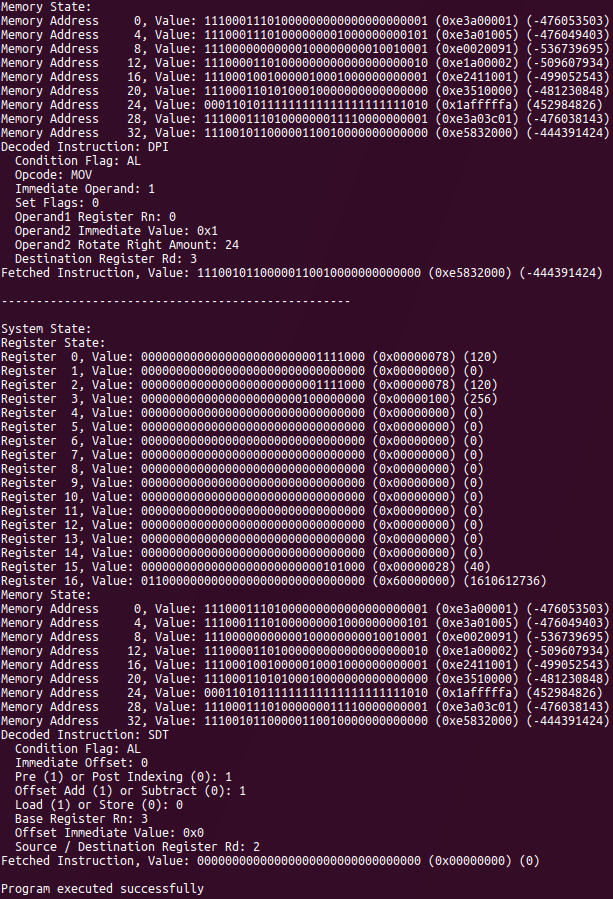
\includegraphics[width=\textwidth]{Presentation/emulate.png}
			\end{figure}
		\end{column}
	\end{columns}
\end{frame}

\begin{frame}
	\frametitle{Terminal-based Game Engine}
	\begin{columns}
		\begin{column}{0.65\textwidth}
			\emph{Makes it easy to write terminal-based games}
			
			In the function template \texttt{init\_game}:
			\begin{enumerate}
				\item Define objects using \texttt{object\_list\_elem\_t}.
				\begin{enumerate}
					\item Type
					\item Position
					\item Velocity
					\item Acceleration
					\item ASCII representation (string, colour, size)
					\item Depth
					\item Pointer to another object
				\end{enumerate}
				\item Create collections of items (using \texttt{object\_list\_t}).
				\item Choose the \texttt{FRAMERATE}.
				\item Set up colour pairs (used by \texttt{ncurses}).
			\end{enumerate}
		\end{column}
		\begin{column}{0.35\textwidth}
			\begin{figure}
				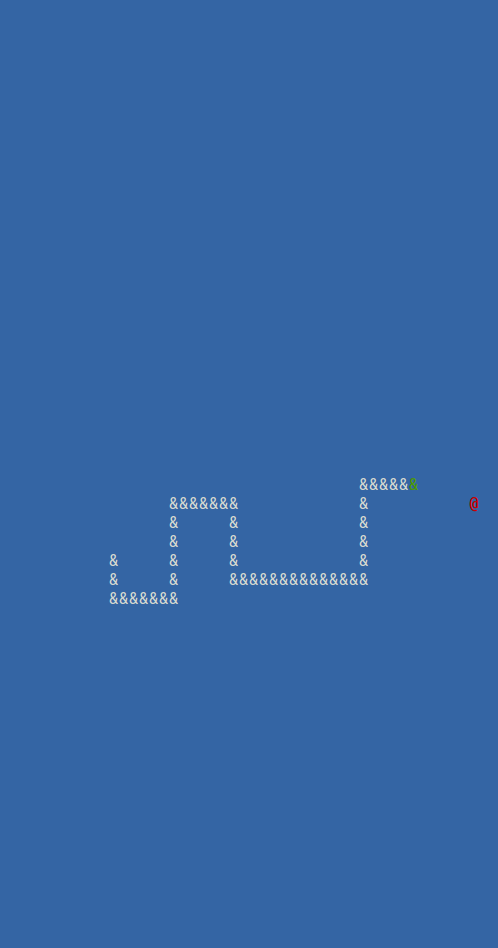
\includegraphics[width=\textwidth]{Presentation/snake.png}
			\end{figure}
		\end{column}
	\end{columns}
\end{frame}

\begin{frame}
\frametitle{Terminal-based Game Engine (continued)}
\begin{columns}
	\begin{column}{0.55\textwidth}
		\begin{figure}
			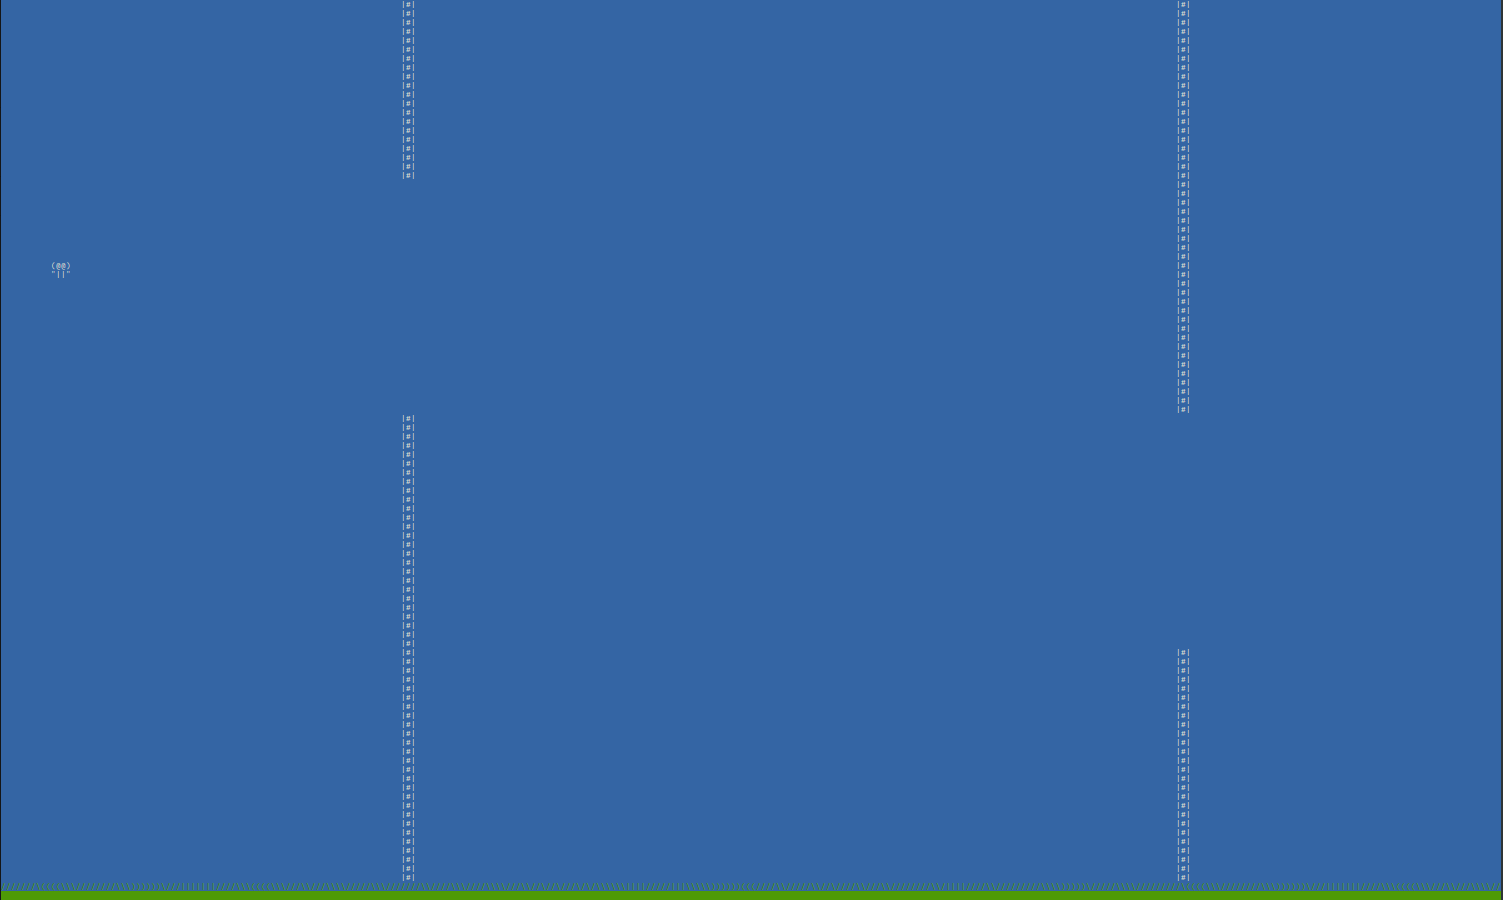
\includegraphics[width=\textwidth]{Presentation/flappy.png}
		\end{figure}
	\end{column}
	\begin{column}{0.45\textwidth}
		Write some simple helper functions to call on objects:
		\begin{enumerate}
			\setcounter{enumi}{3}
			\item E.g. \texttt{move}.
			\item E.g. \texttt{detect\_collision} (can use \texttt{is\_covering}).
		\end{enumerate}
		Complete the main game loop:
		\begin{enumerate}
			\setcounter{enumi}{5}
			\item Use \texttt{for\_all} to call \texttt{move} on objects.
			\item Call \texttt{print\_game}.
			\item Receive input using \texttt{getch}.
			\item Check game logic.
		\end{enumerate}
	\end{column}
\end{columns}
\end{frame}

\begin{frame}
\frametitle{Motion control using OpenCV}
\begin{columns}
	\begin{column}{0.65\textwidth}
		\begin{itemize}
			\item Calibrate engine to users skin colour
			\item Apply threshold to image using skin colour
			\item Median blur to remove noise
			\item Apply hand tracking algorithm
		\end{itemize}
	\end{column}
	\begin{column}{0.35\textwidth}
		\begin{figure}
			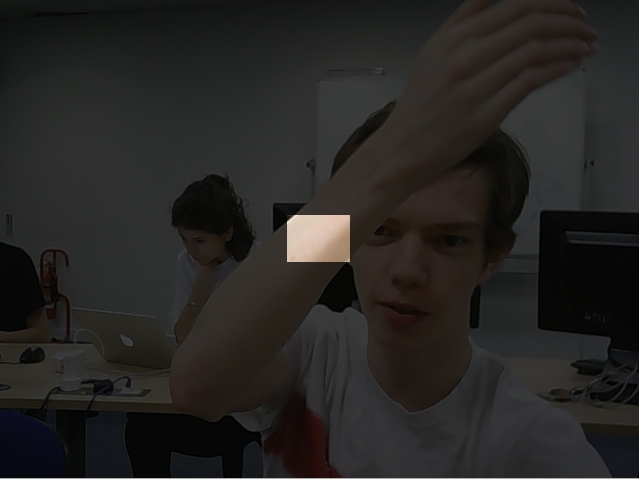
\includegraphics[width=\textwidth]{Presentation/calibration.png}
		\end{figure}
	\end{column}
\end{columns}
\begin{figure}
			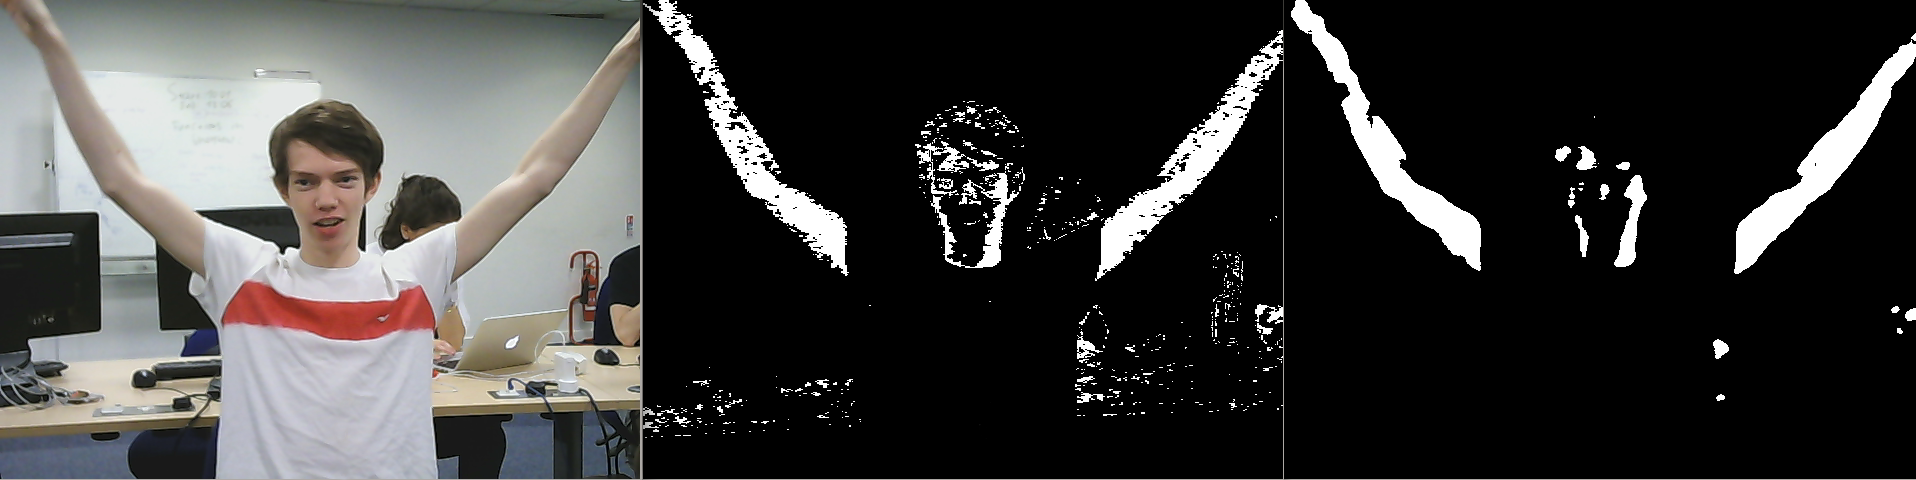
\includegraphics[width=\textwidth]{Presentation/opencv.png}
		\end{figure}
\end{frame}

\begin{frame}
\frametitle{Motion control using OpenCV {hand tracking}}
\begin{itemize}
	\item Two points are initalised in the "guess" position
	\item Update each frame, mvoing away from the centre and towards high density regions of skin
	\item If they wander out of bounds then reposition to the guess points
	\item If the points enter certain regions then we classify this as "left hand up", "right hand down" ...
\end{itemize}
\end{frame}

\begin{frame}
\frametitle{Demonstration}
\begin{itemize}
	\item TODO
\end{itemize}
\end{frame}

\begin{frame}
\frametitle{Testing}
\begin{itemize}
	\item TODO
\end{itemize}
\end{frame}

\begin{frame}
\frametitle{Reflection}
\begin{itemize}
	\item TODO
\end{itemize}
\end{frame}

\end{document}